\documentclass{article}
\usepackage[paperwidth=7.16in,paperheight=4.55in,margin=0.08in]{geometry}
\usepackage{amsmath}
\usepackage{amssymb}
\usepackage{array}
\usepackage{tikz}
\usetikzlibrary{arrows.meta,positioning,calc}
\pagestyle{empty}
\setlength{\parindent}{0pt}

% Restrained journal palette: blue marks complex-valued operations;
% neutral fills keep the figure legible at two-column width.
\definecolor{complexfill}{RGB}{237,246,250}
\definecolor{complexedge}{RGB}{54,102,135}
\definecolor{neutralfill}{RGB}{248,248,247}
\definecolor{neutraledge}{RGB}{105,105,101}
\definecolor{rulegray}{RGB}{170,170,166}
\definecolor{textgray}{RGB}{55,55,53}

\begin{document}
\centering
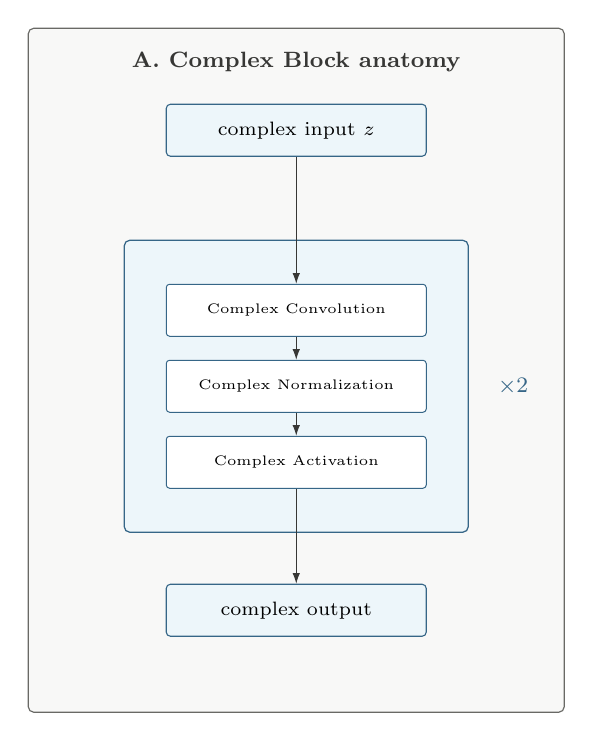
\begin{tikzpicture}[
  x=1in,y=1in,
  font=\scriptsize,
  >=Latex,
  arrow/.style={-{Latex[length=1.35mm,width=0.95mm]},line width=0.34pt,draw=textgray},
  panel/.style={rounded corners=2pt,draw=neutraledge,fill=neutralfill,line width=0.42pt},
  bluebox/.style={rounded corners=1.5pt,draw=complexedge,fill=complexfill,line width=0.40pt,
    align=center,inner sep=2pt},
  opbox/.style={rounded corners=1.2pt,draw=complexedge,fill=white,line width=0.36pt,
    align=center,inner sep=2pt,font=\tiny},
  groupbox/.style={rounded corners=2pt,draw=complexedge,fill=complexfill,line width=0.45pt,
    minimum width=1.72in,minimum height=1.46in},
  paneltitle/.style={font=\footnotesize\bfseries,text=textgray},
  subhead/.style={font=\scriptsize\bfseries,text=complexedge},
  eq/.style={font=\tiny,text=textgray,align=center},
  note/.style={font=\tiny,text=textgray,align=center}
]

% -------------------------------------------------------------------------
% Complex Block anatomy
% -------------------------------------------------------------------------
\node[panel,minimum width=2.68in,minimum height=3.42in] (anatomy) at (0,0.28) {};
\node[paneltitle] at (0,1.82) {A. Complex Block anatomy};

\node[bluebox,minimum width=1.30in,minimum height=0.26in] (zin) at (0,1.48)
  {complex input $z$};
\node[groupbox] (sequence) at (0,0.20) {};
\node[opbox,minimum width=1.30in,minimum height=0.26in] (c1) at (0,0.58)
  {Complex Convolution};
\node[opbox,minimum width=1.30in,minimum height=0.26in] (n1) at (0,0.20)
  {Complex Normalization};
\node[opbox,minimum width=1.30in,minimum height=0.26in] (a1) at (0,-0.18)
  {Complex Activation};
\node[bluebox,minimum width=1.30in,minimum height=0.26in] (zout) at (0,-0.92)
  {complex output};
\foreach \a/\b in {zin/c1,c1/n1,n1/a1,a1/zout}
  {\draw[arrow] (\a.south) -- (\b.north);}
\node[font=\footnotesize\bfseries,text=complexedge,anchor=west] at (0.96,0.20) {$\times 2$};
\end{tikzpicture}

\vspace{0.02in}
\begin{minipage}{7.00in}
\scriptsize
\textbf{Figure 4.} Complex Block anatomy showing two repeated convolution--normalization--activation sequences from complex input to complex output.
\end{minipage}
\end{document}
